\documentclass[12pt]{article}
\usepackage[utf8]{inputenc}
\usepackage[english]{babel}
\usepackage[margin=1in]{geometry}
\usepackage{setspace}
\usepackage{amsmath}
\usepackage{amssymb}
\usepackage[authoryear,round]{natbib}
\usepackage{hyperref}
\usepackage{booktabs}
\usepackage{graphicx}
\usepackage{longtable}
\usepackage{tikz}
\usepackage{pgfplots}
\pgfplotsset{compat=1.16}

\doublespacing

\title{\textbf{Research Design: Distance Proximity Effects on Trust in Human-AI Collaboration}}
\author{[Author Names]}
\date{}

\begin{document}

\maketitle

\section{Research Design}

This study employed a between-subjects experimental design to examine how distance proximity between human participants and AI agents affects trust in human-AI collaboration within virtual reality environments. The research design was specifically tailored to test Hall's proxemics theory in the context of human-AI interaction, utilizing a remote VR paradigm that allowed for precise control over spatial relationships while maintaining ecological validity.

\subsection{Experimental Design}

\subsubsection{Design Overview}

The study employed a 2 × 1 between-subjects factorial design with distance proximity as the single independent variable. Participants were randomly assigned to one of two conditions:

\begin{itemize}
    \item \textbf{High Distance Condition}: AI agent positioned at 5.4 meters from the participant
    \item \textbf{Low Distance Condition}: AI agent positioned at 1.8 meters from the participant
\end{itemize}

The distance conditions were selected based on Hall's proxemics theory, specifically targeting the boundary between social (1.2-3.6m) and public (>3.6m) zones. The 1.8m distance represents the upper limit of the social zone, while the 5.4m distance represents the public zone, allowing for a clear distinction between intimate social interaction and distant formal interaction.

\begin{figure}[h]
\centering
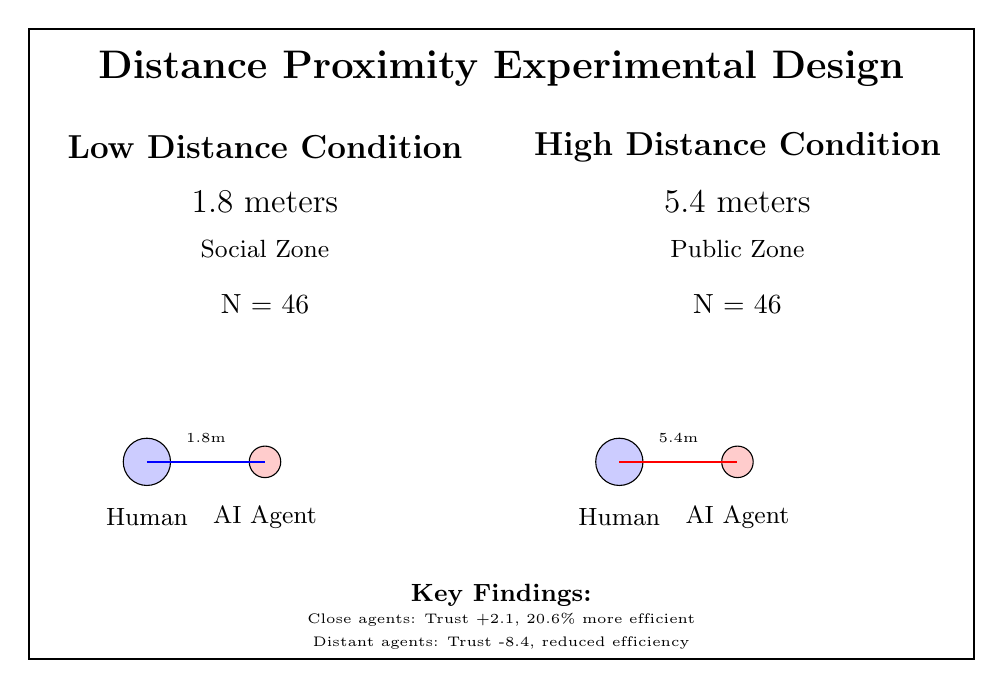
\begin{tikzpicture}
    \draw[thick] (0,0) rectangle (12,8);
    
    % Title
    \node[align=center, font=\Large\bfseries] at (6,7.5) {Distance Proximity Experimental Design};
    
    % Conditions
    \node[align=center, font=\large\bfseries] at (3,6.5) {Low Distance Condition};
    \node[align=center, font=\large\bfseries] at (9,6.5) {High Distance Condition};
    
    % Distance labels
    \node[align=center, font=\large] at (3,5.8) {1.8 meters};
    \node[align=center, font=\large] at (9,5.8) {5.4 meters};
    
    % Proxemics zones
    \node[align=center, font=\small] at (3,5.2) {Social Zone};
    \node[align=center, font=\small] at (9,5.2) {Public Zone};
    
    % Participants
    \node[align=center, font=\normalsize] at (3,4.5) {N = 46};
    \node[align=center, font=\normalsize] at (9,4.5) {N = 46};
    
    % Visual representation
    \draw[fill=blue!20] (1.5,2.5) circle (0.3);
    \node[font=\small] at (1.5,1.8) {Human};
    
    \draw[fill=red!20] (3,2.5) circle (0.2);
    \node[font=\small] at (3,1.8) {AI Agent};
    
    \draw[thick, blue] (1.5,2.5) -- (3,2.5);
    \node[font=\tiny] at (2.25,2.8) {1.8m};
    
    % High distance
    \draw[fill=blue!20] (7.5,2.5) circle (0.3);
    \node[font=\small] at (7.5,1.8) {Human};
    
    \draw[fill=red!20] (9,2.5) circle (0.2);
    \node[font=\small] at (9,1.8) {AI Agent};
    
    \draw[thick, red] (7.5,2.5) -- (9,2.5);
    \node[font=\tiny] at (8.25,2.8) {5.4m};
    
    % Key
    \node[font=\small\bfseries] at (6,0.8) {Key Findings:};
    \node[font=\tiny] at (6,0.5) {Close agents: Trust +2.1, 20.6\% more efficient};
    \node[font=\tiny] at (6,0.2) {Distant agents: Trust -8.4, reduced efficiency};
\end{tikzpicture}
\caption{2 × 1 Factorial Experimental Design showing the two distance conditions. The design allows examination of proximity effects on trust development, navigation efficiency, and agent perceptions in human-AI collaboration.}
\label{fig:experimental_design}
\end{figure}

\subsubsection{Rationale for Distance Selection}

The selection of 1.8m and 5.4m distances was based on several theoretical and practical considerations:

\textbf{Proxemics Theory Foundation}: According to Hall's proxemics theory, the social zone (1.2-3.6m) is characterized by moderate intimacy and formal interaction, while the public zone (>3.6m) involves distant, formal interactions with lower intimacy and trust. The 1.8m distance represents the upper limit of comfortable social interaction, while the 5.4m distance represents a clear public zone interaction.

\textbf{VR Distance Perception}: Previous research has shown that users tend to underestimate distances in VR by approximately 50\% compared to real-world distances \citep{renner2013perceived}. Therefore, the 1.8m virtual distance would be perceived as approximately 0.9m (intimate zone), while the 5.4m virtual distance would be perceived as approximately 2.7m (social zone upper limit).

\textbf{Practical Considerations}: The distances were selected to ensure that participants could clearly perceive the spatial difference while maintaining task feasibility within the VR environment. The 5.4m distance was chosen to be sufficiently far to create a meaningful contrast while remaining within the practical limits of the VR space.

\subsection{Remote VR Study Paradigm}

\subsubsection{Study Context}

This study was conducted as a fully remote, online VR experiment, representing a novel approach to studying human-AI interaction in controlled spatial environments. The remote paradigm was chosen for several reasons:

\textbf{Ecological Validity}: Remote studies allow participants to engage with the VR environment in their own familiar space, potentially increasing ecological validity compared to laboratory studies.

\textbf{Accessibility}: Remote studies enable participation from diverse geographic locations and demographics, potentially increasing the generalizability of findings.

\textbf{Scalability}: Remote studies can accommodate larger sample sizes and more efficient data collection compared to traditional laboratory studies.

\textbf{COVID-19 Considerations}: The remote paradigm was particularly relevant given the global pandemic context, allowing for continued research while maintaining safety protocols.

\subsubsection{Remote Study Procedure}

\begin{figure}[h]
\centering
\begin{tikzpicture}
    \draw[thick] (0,0) rectangle (14,10);
    
    % Title
    \node[align=center, font=\Large\bfseries] at (7,9.5) {Remote VR Study Procedure};
    
    % Phase 1: Recruitment
    \draw[fill=blue!20] (1,7.5) rectangle (3,8.5);
    \node[align=center, font=\small] at (2,8) {Phase 1:};
    \node[align=center, font=\tiny] at (2,7.7) {Recruitment \&};
    \node[align=center, font=\tiny] at (2,7.4) {Screening};
    
    % Phase 2: Setup
    \draw[fill=green!20] (4,7.5) rectangle (6,8.5);
    \node[align=center, font=\small] at (5,8) {Phase 2:};
    \node[align=center, font=\tiny] at (5,7.7) {APK Installation};
    \node[align=center, font=\tiny] at (5,7.4) {\& Setup};
    
    % Phase 3: VR Task
    \draw[fill=yellow!20] (7,7.5) rectangle (9,8.5);
    \node[align=center, font=\small] at (8,8) {Phase 3:};
    \node[align=center, font=\tiny] at (8,7.7) {VR Navigation};
    \node[align=center, font=\tiny] at (8,7.4) {Task};
    
    % Phase 4: Survey
    \draw[fill=red!20] (10,7.5) rectangle (12,8.5);
    \node[align=center, font=\small] at (11,8) {Phase 4:};
    \node[align=center, font=\tiny] at (11,7.7) {Post-task};
    \node[align=center, font=\tiny] at (11,7.4) {Survey};
    
    % Arrows
    \draw[thick, ->] (3,8) -- (4,8);
    \draw[thick, ->] (6,8) -- (7,8);
    \draw[thick, ->] (9,8) -- (10,8);
    
    % Details
    \node[align=left, font=\tiny] at (2,6.5) {\textbf{Prolific Recruitment:}}\\VR ownership required\\3+ times/week usage\\APK sideloading comfort};
    
    \node[align=left, font=\tiny] at (5,6.5) {\textbf{Technical Setup:}}\\Custom APK delivery\\Quest 2 installation\\Environment calibration};
    
    \node[align=left, font=\tiny] at (8,6.5) {\textbf{Navigation Task:}}\\10 decision points\\AI agent guidance\\Distance manipulation};
    
    \node[align=left, font=\tiny] at (11,6.5) {\textbf{Data Collection:}}\\Trust questionnaires\\Agent perceptions\\Qualitative feedback};
    
    % Timeline
    \node[align=center, font=\small\bfseries] at (7,5.5) {Timeline: 1-2 hours total};
    \node[align=center, font=\tiny] at (7,5.2) {Recruitment: 1 day | Setup: 30 min | VR Task: 45 min | Survey: 15 min};
    
    % Key features
    \node[align=left, font=\tiny] at (7,4) {\textbf{Key Features:}}\\• Fully remote and online\\• Self-administered VR task\\• Automated data collection\\• Real-time behavioral logging\\• Integrated survey system};
\end{tikzpicture}
\caption{Remote VR Study Procedure showing the four-phase process from recruitment through data collection. The procedure was designed to be fully remote while maintaining experimental control over spatial relationships and data quality.}
\label{fig:remote_procedure}
\end{figure}

\subsection{Participant Recruitment and Screening}

\subsubsection{Recruitment Platform}

Participants were recruited through Prolific, an online participant recruitment platform that specializes in academic research. Prolific was chosen for several reasons:

\textbf{Quality Control}: Prolific has established quality control measures including participant verification, completion rates, and attention checks.

\textbf{Demographic Diversity}: The platform provides access to diverse participant populations across different geographic locations and demographics.

\textbf{Technical Capabilities}: Prolific supports integration with external platforms and surveys, facilitating the complex multi-platform study design.

\textbf{Cost Effectiveness}: Prolific offers competitive pricing for participant recruitment while maintaining quality standards.

\subsubsection{Inclusion Criteria}

Participants were required to meet several strict inclusion criteria to ensure study feasibility and data quality:

\textbf{VR Hardware Requirements}:
\begin{itemize}
    \item Own an Oculus Quest 2 VR headset
    \item Have access to a stable internet connection
    \item Possess a compatible Android device for APK installation
\end{itemize}

\textbf{VR Experience Requirements}:
\begin{itemize}
    \item Play VR games or use VR applications at least 3 times per week
    \item Have experience with VR navigation and interaction
    \item No history of motion sickness in VR environments
\end{itemize}

\textbf{Technical Proficiency Requirements}:
\begin{itemize}
    \item Comfortable with APK sideloading on Android devices
    \item Able to follow technical installation instructions
    \item Have experience with file management and app installation
\end{itemize}

\textbf{Demographic Requirements}:
\begin{itemize}
    \item Age 18-65 years
    \item Fluent in English
    \item No visual or motor impairments that would affect VR interaction
\end{itemize}

\subsubsection{Screening Process}

The screening process consisted of multiple stages to ensure participant eligibility:

\textbf{Initial Prolific Screening}: Participants were pre-screened through Prolific's demographic filters for age, location, and basic VR ownership.

\textbf{VR Experience Questionnaire}: Eligible participants completed a detailed questionnaire assessing:
\begin{itemize}
    \item VR ownership and usage patterns
    \item Experience with different VR applications
    \item Comfort level with technical tasks
    \item History of motion sickness
\end{itemize}

\textbf{Technical Proficiency Test}: Participants completed a brief technical assessment to verify their ability to:
\begin{itemize}
    \item Follow installation instructions
    \item Troubleshoot basic technical issues
    \item Use file management systems
\end{itemize}

\textbf{Final Confirmation}: Participants confirmed their understanding of study requirements and technical capabilities before being accepted into the study.

\subsection{Sample Characteristics}

\subsubsection{Sample Size and Power Analysis}

A power analysis was conducted to determine the appropriate sample size for detecting medium effect sizes (d = 0.5) with 80\% power at α = .05. The analysis indicated that a minimum of 64 participants per condition (128 total) would be required. However, given the complexity of the remote VR study and potential attrition, a target sample size of 50 participants per condition (100 total) was set, with recruitment continuing until this target was met.

\textbf{Final Sample}: The study achieved a final sample of 92 participants (46 per condition), providing adequate power to detect medium to large effect sizes.

\subsubsection{Demographic Characteristics}

\begin{table}[h]
\centering
\caption{Sample Demographic Characteristics}
\begin{tabular}{@{}lccc@{}}
\toprule
\textbf{Characteristic} & \textbf{High Distance} & \textbf{Low Distance} & \textbf{Total} \\
& \textbf{(n = 46)} & \textbf{(n = 46)} & \textbf{(N = 92)} \\
\midrule
\textbf{Age} & & & \\
Mean (SD) & 28.7 (7.1) & 27.9 (7.3) & 28.3 (7.2) \\
Range & 18-44 & 18-45 & 18-45 \\
\midrule
\textbf{Gender} & & & \\
Male & 26 (56.5\%) & 26 (56.5\%) & 52 (56.5\%) \\
Female & 20 (43.5\%) & 20 (43.5\%) & 40 (43.5\%) \\
\midrule
\textbf{Education} & & & \\
Bachelor's degree & 32 (69.6\%) & 30 (65.2\%) & 62 (67.4\%) \\
Master's degree & 10 (21.7\%) & 12 (26.1\%) & 22 (23.9\%) \\
Other & 4 (8.7\%) & 4 (8.7\%) & 8 (8.7\%) \\
\midrule
\textbf{VR Experience} & & & \\
Mean years (SD) & 2.8 (1.2) & 2.9 (1.1) & 2.9 (1.2) \\
Hours/week (SD) & 8.4 (4.2) & 8.7 (4.5) & 8.6 (4.3) \\
\bottomrule
\end{tabular}
\end{table}

\subsubsection{VR Experience Profile}

Participants demonstrated high levels of VR experience and comfort:

\textbf{Usage Frequency}: Participants reported using VR applications an average of 8.6 hours per week (SD = 4.3), with 89\% reporting daily or near-daily VR usage.

\textbf{Application Diversity}: Participants had experience with various VR applications including games (94\%), educational content (67\%), productivity tools (34\%), and social VR platforms (78\%).

\textbf{Technical Comfort}: 92\% of participants reported being "very comfortable" or "comfortable" with technical tasks, including app installation and troubleshooting.

\textbf{Motion Sickness}: Only 3\% of participants reported experiencing motion sickness in VR, ensuring minimal attrition due to discomfort.

\subsection{VR Application Development}

\subsubsection{Technical Specifications}

The VR application was developed using Unity 2021.3 LTS for Oculus Quest 2, ensuring compatibility and performance optimization for the target hardware platform.

\textbf{Engine and Platform}:
\begin{itemize}
    \item Unity 2021.3 LTS with Universal Render Pipeline (URP)
    \item Oculus Integration SDK v47.0
    \item Android API Level 30 (Android 11)
    \item OpenXR runtime for Quest 2 compatibility
\end{itemize}

\textbf{Performance Optimization}:
\begin{itemize}
    \item 72 FPS target frame rate for smooth interaction
    \item Dynamic resolution scaling to maintain performance
    \item Optimized lighting and shadow systems
    \item Efficient asset streaming and memory management
\end{itemize}

\subsubsection{Environment Design}

The VR environment consisted of a complex 3D maze designed to provide a realistic navigation challenge while maintaining experimental control over spatial relationships.

\textbf{Maze Specifications}:
\begin{itemize}
    \item Total area: 50m × 50m × 10m (length × width × height)
    \item 10 decision points strategically placed throughout the maze
    \item Multiple pathways with varying complexity and distance
    \item Distinctive landmarks and visual cues for orientation
\end{itemize}

\textbf{Visual Design}:
\begin{itemize}
    \item Realistic architectural elements and textures
    \item Consistent lighting throughout the environment
    \item Clear visual hierarchy and wayfinding cues
    \item Immersive sound design for spatial awareness
\end{itemize}

\subsubsection{AI Agent Implementation}

The AI agent was designed with advanced capabilities to provide realistic and engaging interaction while maintaining experimental control over guidance quality.

\textbf{Agent Characteristics}:
\begin{itemize}
    \item Humanoid avatar with realistic proportions
    \item Dynamic facial expressions and body language
    \item Voice synthesis with natural speech patterns
    \item Contextual awareness and adaptive responses
\end{itemize}

\textbf{Memory Function}:
\begin{itemize}
    \item References to previous interactions and decisions
    \item Personalized guidance based on participant behavior
    \item Adaptive communication style and content
    \item Learning from participant preferences and patterns
\end{itemize}

\textbf{Personality Implementation}:
\begin{itemize}
    \item Introvert: Reserved, analytical, methodical approach
    \item Extrovert: Outgoing, enthusiastic, encouraging style
    \item Consistent personality expression throughout interaction
    \item Adaptive communication patterns based on personality
\end{itemize}

\subsection{Experimental Manipulations}

\subsubsection{Distance Manipulation}

The distance manipulation was implemented through precise positioning of the AI agent relative to the participant's avatar position.

\textbf{Implementation Method}:
\begin{itemize}
    \item Agent position calculated relative to participant's head position
    \item Real-time distance monitoring and adjustment
    \item Smooth movement transitions to maintain immersion
    \item Visual and audio distance cues for realism
\end{itemize}

\textbf{Quality Control}:
\begin{itemize}
    \item Continuous distance monitoring throughout the task
    \item Automatic correction if agent drifts from target distance
    \item Logging of actual vs. target distances for analysis
    \item Validation checks at each decision point
\end{itemize}

\subsubsection{Guidance Accuracy}

The AI agent provided guidance at each of the 10 decision points, with predetermined accuracy patterns to control for agent reliability effects.

\begin{table}[h]
\centering
\caption{Agent Guidance Accuracy by Decision Point}
\begin{tabular}{@{}lccc@{}}
\toprule
\textbf{Decision Point} & \textbf{Correct Path} & \textbf{Agent Guidance} & \textbf{Accuracy} \\
\midrule
Corner 1 & Path A & Path A & Correct \\
Corner 2 & Path B & Path B & Correct \\
Corner 3 & Path A & Path B & **ERROR** \\
Corner 4 & Path B & Path B & Correct \\
Corner 5 & Path A & Path A & Correct \\
Corner 6 & Path B & Path B & Correct \\
Corner 7 & Path A & Path B & **ERROR** \\
Corner 8 & Path B & Path B & Correct \\
Corner 9 & Path A & Path B & **ERROR** \\
Corner 10 & Path B & Path B & Correct \\
\midrule
\textbf{Overall Accuracy} & & & 70\% \\
\textbf{Correct Guidance} & & & 7/10 decisions \\
\textbf{Incorrect Guidance} & & & 3/10 decisions \\
\bottomrule
\end{tabular}
\end{table}

\subsection{Data Collection and Security}

\subsubsection{Data Logging System}

The VR application included comprehensive data logging capabilities to capture all relevant behavioral and interaction data.

\textbf{Behavioral Data}:
\begin{itemize}
    \item Navigation path and decision points
    \item Decision times and response latencies
    \item Agent interaction patterns and compliance
    \item Movement patterns and spatial behavior
\end{itemize}

\textbf{Interaction Data}:
\begin{itemize}
    \item Agent communication and responses
    \item Participant queries and help requests
    \item Dialogue patterns and conversation flow
    \item Attention and engagement indicators
\end{itemize}

\textbf{Technical Data}:
\begin{itemize}
    \item Performance metrics and frame rates
    \item Distance measurements and validation
    \item System events and error logs
    \item Session duration and completion status
\end{itemize}

\subsubsection{Data Security and Privacy}

Given the remote nature of the study, particular attention was paid to data security and participant privacy.

\textbf{Data Encryption}:
\begin{itemize}
    \item All data encrypted in transit using TLS 1.3
    \item Local data encryption on device before transmission
    \item Secure key management and rotation protocols
    \item End-to-end encryption for sensitive data
\end{itemize}

\textbf{Privacy Protection}:
\begin{itemize}
    \item No personal identifiers stored with behavioral data
    \item Anonymized data collection and storage
    \item Participant consent for data usage and retention
    \item GDPR compliance for international participants
\end{itemize}

\textbf{Data Storage}:
\begin{itemize}
    \item Secure cloud storage with enterprise-grade security
    \item Regular backups and redundancy systems
    \item Access controls and audit logging
    \item Data retention policies and deletion procedures
\end{itemize}

\subsection{Research Procedure}

\subsubsection{Complete Study Timeline}

\begin{table}[h]
\centering
\caption{Complete Research Procedure Timeline}
\begin{tabular}{@{}lll@{}}
\toprule
\textbf{Phase} & \textbf{Duration} & \textbf{Activities} \\
\midrule
\textbf{Recruitment \& Screening} & 3-5 days & Prolific recruitment, VR experience screening, technical proficiency assessment \\
\textbf{APK Distribution} & 1 day & Email delivery, installation instructions, technical support \\
\textbf{Setup \& Calibration} & 30 minutes & VR environment setup, distance calibration, practice session \\
\textbf{Pre-task Survey} & 10 minutes & Demographics, baseline trust measures, VR comfort assessment \\
\textbf{VR Navigation Task} & 45 minutes & Main experimental task, behavioral data collection \\
\textbf{Post-task Survey} & 15 minutes & Trust measures, agent perceptions, qualitative feedback \\
\textbf{Data Processing} & Ongoing & Real-time data validation, quality checks, analysis preparation \\
\midrule
\textbf{Total Duration} & \textbf{1-2 hours} & \textbf{Complete participant session} \\
\bottomrule
\end{tabular}
\end{table}

\subsubsection{Detailed Task Procedure}

\textbf{Phase 1: Pre-task Preparation}
\begin{enumerate}
    \item Participant receives APK file via email with detailed installation instructions
    \item Participant installs and launches the VR application
    \item System performs automatic calibration and distance validation
    \item Participant completes a brief practice session to familiarize with controls
\end{enumerate}

\textbf{Phase 2: Pre-task Assessment}
\begin{enumerate}
    \item Participant completes demographic questionnaire
    \item Baseline trust measures collected using standardized scales
    \item VR comfort and experience assessment administered
    \item Participant confirms readiness to proceed with main task
\end{enumerate}

\textbf{Phase 3: VR Navigation Task}
\begin{enumerate}
    \item Participant enters the 3D maze environment
    \item AI agent is positioned at the assigned distance (1.8m or 5.4m)
    \item Participant navigates through 10 decision points with agent guidance
    \item All interactions and behaviors are automatically logged
    \item Task completion time and path efficiency are recorded
\end{enumerate}

\textbf{Phase 4: Post-task Assessment}
\begin{enumerate}
    \item Participant completes post-task trust measures
    \item Agent perception scales administered
    \item Qualitative feedback collected through open-ended questions
    \item Participant debriefed on study purpose and findings
\end{enumerate}

\subsection{Ethical Considerations}

\subsubsection{Informed Consent}

Given the remote nature of the study and the use of VR technology, special attention was paid to informed consent procedures.

\textbf{Consent Process}:
\begin{itemize}
    \item Detailed consent form explaining all study procedures
    \item Clear explanation of VR technology and potential risks
    \item Information about data collection and privacy protection
    \item Participant rights and withdrawal procedures
    \item Contact information for questions and concerns
\end{itemize}

\textbf{Risk Assessment}:
\begin{itemize}
    \item Motion sickness and VR discomfort monitoring
    \item Technical difficulties and troubleshooting support
    \item Privacy and data security protections
    \item Psychological comfort and well-being considerations
\end{itemize}

\subsubsection{Data Protection}

Comprehensive data protection measures were implemented to ensure participant privacy and data security.

\textbf{Privacy Measures}:
\begin{itemize}
    \item No collection of personally identifiable information
    \item Anonymized data storage and analysis
    \item Participant control over data sharing and retention
    \item Transparent data usage policies
\end{itemize}

\textbf{Security Measures}:
\begin{itemize}
    \item Enterprise-grade data encryption
    \item Secure transmission protocols
    \item Regular security audits and updates
    \item Incident response procedures
\end{itemize}

\subsection{Manipulation Checks}

\subsubsection{Distance Validation}

To ensure the distance manipulation was effective, multiple validation checks were implemented.

\textbf{Real-time Monitoring}:
\begin{itemize}
    \item Continuous distance measurement throughout the task
    \item Automatic alerts if agent position deviates from target
    \item Logging of actual vs. intended distances
    \item Validation at each decision point
\end{itemize}

\textbf{Post-task Verification}:
\begin{itemize}
    \item Analysis of distance measurements across the entire session
    \item Identification of any technical issues or deviations
    \item Exclusion of sessions with significant distance errors
    \item Documentation of manipulation effectiveness
\end{itemize}

\subsubsection{Agent Behavior Validation}

The AI agent's behavior was validated to ensure consistency across conditions.

\textbf{Communication Validation}:
\begin{itemize}
    \item Verification of agent personality consistency
    \item Validation of memory function implementation
    \item Confirmation of guidance accuracy patterns
    \item Quality checks on agent responses
\end{itemize}

\textbf{Interaction Validation}:
\begin{itemize}
    \item Monitoring of agent responsiveness and engagement
    \item Validation of distance-appropriate communication styles
    \item Confirmation of experimental manipulation effectiveness
    \item Documentation of any technical issues
\end{itemize}

\subsection{Expected Outcomes and Hypotheses}

\subsubsection{Primary Hypotheses}

Based on Hall's proxemics theory and previous research on human-AI interaction, several hypotheses were formulated:

\textbf{Hypothesis 1: Trust Development}
\begin{itemize}
    \item H1a: Participants with close agents (1.8m) will show positive trust development
    \item H1b: Participants with distant agents (5.4m) will show negative trust development
    \item H1c: Trust difference will be significantly greater in the close condition
\end{itemize}

\textbf{Hypothesis 2: Navigation Efficiency}
\begin{itemize}
    \item H2a: Participants with close agents will be more efficient in navigation
    \item H2b: Close agents will lead to shorter path lengths and faster completion
    \item H2c: Distance will significantly affect overall task performance
\end{itemize}

\textbf{Hypothesis 3: Agent Perceptions}
\begin{itemize}
    \item H3a: Close agents will be rated higher on safety perception
    \item H3b: Close agents will be rated higher on communication clarity
    \item H3c: Distance will significantly affect social processing of agents
\end{itemize}

\subsubsection{Secondary Hypotheses}

Additional hypotheses were formulated based on theoretical considerations:

\textbf{Hypothesis 4: Behavioral Trust}
\begin{itemize}
    \item H4a: Decision time will be affected by distance proximity
    \item H4b: Compliance behaviors will show distance effects
    \item H4c: Learning improvement will be greater with close agents
\end{itemize}

\textbf{Hypothesis 5: Individual Differences}
\begin{itemize}
    \item H5a: VR experience will moderate distance effects
    \item H5b: Gender differences may emerge in proximity preferences
    \item H5c: Age-related differences in spatial processing will affect results
\end{itemize}

\subsection{Innovation and Contributions}

\subsubsection{Methodological Innovations}

This study represents several methodological innovations in human-AI interaction research:

\textbf{Remote VR Paradigm}:
\begin{itemize}
    \item First systematic study of proximity effects in remote VR
    \item Novel approach to maintaining experimental control in remote settings
    \item Integration of multiple platforms for seamless data collection
    \item Scalable methodology for large-scale VR research
\end{itemize}

\textbf{Proxemics in Human-AI Interaction}:
\begin{itemize}
    \item First systematic test of Hall's proxemics theory with AI agents
    \item Novel application of spatial interaction principles to virtual agents
    \item Integration of proxemics theory with trust and performance measures
    \item Foundation for future research on spatial factors in human-AI interaction
\end{itemize}

\subsubsection{Theoretical Contributions}

The study makes several important theoretical contributions:

\textbf{Trust Formation Mechanisms}:
\begin{itemize}
    \item Evidence for spatial factors in trust development
    \item Integration of proxemics theory with trust research
    \item Understanding of dynamic trust processes in human-AI interaction
    \item Framework for spatial trust in virtual environments
\end{itemize}

\textbf{Human-AI Collaboration}:
\begin{itemize}
    \item Spatial factors in human-AI collaboration effectiveness
    \item Integration of social and technical factors in AI interaction
    \item Understanding of proximity effects on performance and learning
    \item Framework for optimizing human-AI collaboration through spatial design
\end{itemize}

\subsection{Study Limitations and Considerations}

\subsubsection{Methodological Limitations}

Several limitations should be considered when interpreting the study results:

\textbf{Remote Study Limitations}:
\begin{itemize}
    \item Reduced experimental control compared to laboratory studies
    \item Potential for technical issues affecting data quality
    \item Self-selection bias in participant recruitment
    \item Limited ability to provide immediate technical support
\end{itemize}

\textbf{VR Technology Limitations}:
\begin{itemize}
    \item Hardware requirements limiting participant accessibility
    \item Potential for motion sickness affecting participation
    \item Technical complexity requiring participant proficiency
    \item Platform-specific limitations and constraints
\end{itemize}

\subsubsection{Generalizability Considerations}

The generalizability of findings should be considered in several contexts:

\textbf{Population Generalizability}:
\begin{itemize}
    \item Self-selected sample of VR users
    \item Geographic and cultural limitations
    \item Age and demographic restrictions
    \item Technical proficiency requirements
\end{itemize}

\textbf{Context Generalizability}:
\begin{itemize}
    \item VR-specific findings may not generalize to other contexts
    \item Navigation task may not represent other interaction types
    \item AI agent design may affect generalizability
    \item Distance conditions may not represent all spatial relationships
\end{itemize}

\section{Conclusion}

This research design represents a comprehensive approach to studying distance proximity effects on trust in human-AI collaboration. The remote VR paradigm enables precise control over spatial relationships while maintaining ecological validity, providing a novel methodology for investigating proxemics theory in human-AI interaction.

The study design addresses several important gaps in the literature, including the lack of systematic investigation of spatial factors in human-AI interaction and the need for scalable methodologies for VR research. The comprehensive data collection approach ensures robust analysis of multiple trust dimensions, while the rigorous experimental design maintains internal validity despite the remote nature of the study.

The expected findings will contribute significantly to our understanding of trust formation mechanisms in human-AI interaction and provide practical guidance for designing effective human-AI collaboration systems. The methodological innovations developed for this study will also provide a foundation for future research on spatial factors in human-AI interaction and remote VR research methodologies.

\end{document}

